% !TEX spellcheck = en
\documentclass[main.tex]{subfiles} 

\begin{document}

\section{Visualization of Tensor Fields : Current State}
\label{sec:3}


Techniques for tensor field visualization can be viewed as two distinct methods : indirect and 
direct visualization methods. Direct visualization of tensor fields is accomplished with tensor
glyphs; ellipsoids that are formed by the eigenvalues of the tensor field, or by drawing integral 
lines or surfaces. The purpose is to depict full information contained in the field 
\cite{BH06}, \cite{KMW05}, \cite{HFH04}, \cite{FA15}. Indirect methods usually entail the 
extraction of of spesific structural features from the tensor field, like for example topological
features \cite{TS03}, \cite{TSH01}, \cite{TZP06}. In this thesis, our main focus will be direct
visualization methods, with emphasis on integration methods.

\subsection{Direct Visualization Methods}
\subsubsection{Hyperstreamlines}
A second order symmetric tensor in $\mathbf{R}^3$ has six independent elements or components.
We can reduce this number down to three by performing an eigendecomposition of the tensor, 
resulting in three real eigenvalues. Selecting one of these (usually either the major or the minor 
eigenvalue), we can use it's corresponding eigenvector as the direction for the so-called 
hyperstreamline trajectories, which in $\mathbf{R}^3$ are tube like structures
where the other eigenvalues determine the thickness of the trajectories. They show, for example 
how forces are transmitted in a stress-tensor field and how momentum is transferred in a 
momentum-flux-density tensor field. Delmarcelle and Hesselberg, \cite{DH92}, were first to 
introduce the notion of hyperstreamlines. The issue with hyperstreamlines are the same as
we find with streamlines for depiction of vector fields, or isosurfaces for scalar fields; 
occlusion and seeding. In addition, we need to handle degenerate points (similar to the notion
of critical points in a vector field, where in the case of tensors, the degenerate points
occur when at least two of the eigenvalues are equal.).

In \cite{DH93}, Delmarcelle and Hessellink suggest a simply way of handling degenerate 
points (by simply ignoring them). By assuming that the tensor field is smooth, we can then assume 
that the direction of the eigenvector is not likely to vary abruptly (i.e vary more than some 
user defined angle) in between grid points. If, however, the direction changes abruptly, then 
it is reasonable to assume that the hyperstreamline has crossed a degeneracy. To handle this, we 
can simply jump over this point and continue integrating along the direction of the eigenvector. 
Further, we can also keep a track over the transverse eigenvalues to make sure that, where they 
vanish, we can still include the singularities of the cross-section of the hyperstreamline.


\subsubsection{Tensor Glyphs}
The traditional approach to direct visualization of symmetric second order tensor fields
in $\mathbf{R}^2$ and $\mathbf{R}^3$ have been so-called tensor glyphs. This technique 
has been employed heavily for medical imaging, depicting e.g. \hspace{-1mm}diffusion
tensor. Diffusion tensor imaging (DTI) provides information about the diffusion properties 
of water molecules in brain tissue (which differs for gray matter and white matter). Within 
white matter the motion of water molecules is restricted in directions that are perpendicular 
to the fiber tracts. Because of the physical properties of white matter, DTI can be used 
to investigate white matter in the brain. It's main clinical application has been in the 
study and treatment of neurological disorders, such as schizophrenia. DTI makes it 
possible to evaluate the connectivity and coherence of white matter fiber tract, which are 
tought to be abnormal in schizophrenia \cite{KMW05}. The diffusion tensor is a second 
order symmetric tensor in $\mathbf{R}^3$. The tensor is visualized as an ellipsoid, with 
the longest axis pointing toward the principal direction, i.e the major eigenvector. The 
shape of the tensor depends upon the strength of the diffusion along the three 
eigenvectors.

\begin{figure}[H]
\centering
\label{fig:basic_glyphs}
	\subfloat[Three basic diffusion tensor shapes.]
		    {{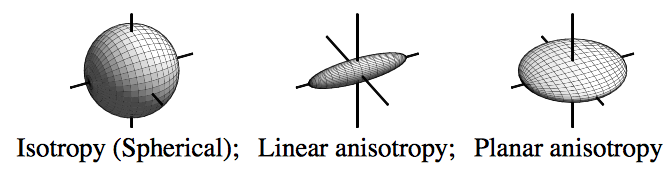
\includegraphics[scale=0.25,natwidth=668,natheight=176]				
		    {../figures/basic_diffusion_glyphs.png}}}
	\qquad
	\subfloat[Linear, planar and isotropic shapes defined by eigenvalues.]	
		     {{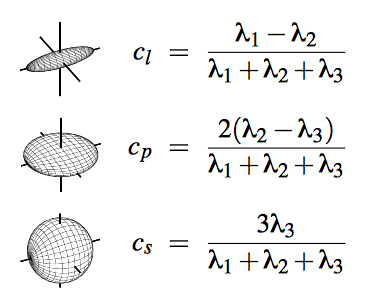
\includegraphics[scale=0.35,natwidth=368,natheight=306]
		     {../figures/glyphs_with_eigenvalues.png}}}
	\caption[Linear, planar and isotropic shapes defined by eigenvalues.]{Linear, planar and isotropic shapes defined by eigenvalues. Picture taken from \cite{Kin04}.}     
\end{figure}

\subsubsection{Asymmetric tensors fields}

We can always describe any (of either covariant or contravariant type) second order tensor 
by the sum of their symmetric and anti-symmetric components. For a second-order tensor of type (2,0), 
we can write it as
\begin{align}\label{eq:decomp}
S_{ij} = \frac{1}{2}\left(S_{ij} + S_{ji}\right) + \frac{1}{2}\left(S_{ij} - S_{ji}\right) 
\end{align}
A physical example for this case is the gradient of a velocity field, $\nabla \mathbf{v}$. If we 
denote the components of $\mathbf{v}$ as $(v_i)$, then we can write the gradient as
\begin{align}\label{eq:gradv}
\nabla \mathbf{v} &=
\begin{bmatrix}
    \frac{\partial v_1}{\partial x^1} & \frac{\partial v_2}{\partial x^1} & \frac{\partial v_3}{\partial x^1}\\\\
    \frac{\partial v_1}{\partial x^2} & \frac{\partial v_2}{\partial x^2} & \frac{\partial v_3}{\partial x^2}\\\\
    \frac{\partial v_1}{\partial x^3} & \frac{\partial v_1}{\partial x^3} & \frac{\partial v_3}{\partial x^3}
\end{bmatrix},
\end{align}
or using index form we can write the components as $\partial v_i/\partial x^j$. Using the above 
notation \eqref{eq:decomp}, we can decompose \eqref{eq:gradv} as 
\begin{align*}
\frac{\partial v_i}{\partial x^j} = 
\frac{1}{2}\left(\frac{\partial v_i}{\partial x^j} + \frac{\partial v_j}{\partial x^i}\right) + 
\frac{1}{2}\left(\frac{\partial v_i}{\partial x^j}  - \frac{\partial v_j}{\partial x^i}\right) 
\end{align*}
The symmetric part is the sum of the Jacobian and transpose of the Jacobian, also refered to as
the \emph{rate of strain tensor}. The diagonal entries are the normal strain rates and the off-diagonal
entries are the shear strain rates.

We can associate a vector $\omega_i$, 
\begin{align*}
\omega = 
\begin{bmatrix}
\omega_1\\
\omega_2\\
\omega_3\\
\end{bmatrix} =
\begin{bmatrix}
\frac{\partial v_3}{\partial x^2} - \frac{\partial v_2}{\partial x^3}\\
\frac{\partial v_1}{\partial x^3} - \frac{\partial v_3}{\partial x^1}\\
\frac{\partial v_2}{\partial x^1} - \frac{\partial v_1}{\partial x^2}
\end{bmatrix}
\end{align*}
with an anti-symmetric tensor defined by
\begin{align*}
R \equiv
\begin{bmatrix}
0  & -\omega_3 & \omega_2\\
\omega_3 & 0 & -\omega_1\\
-\omega_2 & \omega_1 & 0
\end{bmatrix}
\end{align*}
where they are related as
\begin{align*}
R_{ij} = -e_{ijk}\omega_k,\\
\omega_k = -\frac{1}{2}e_{ijk}R_{ij}.
\end{align*}
R is called the \emph{Rotation tensor}.

We can therefore represent the anti-symmetric part as a vector and thereby employ techniques
from vector field visualization. For the symmetric part of the tensor, we can perform an 
eigendecomposition. Which permits us to represent the tensor by it's eigenvectors and their 
corresponding eigenvalues. Delmarcelle and Hesselberg \cite{DH92} were first to decompose 2D 
symmetric tensors of type (2,0) in such a manner.

\subsubsection{The Geodesic Differential Equations}
In Euclidean space, $\mathbf{R}^3$, the distance between two points $(x_1,x_2,x_3)$ and
$(y_1,y_2,y_3)$ is given as $d^2 = |x_i - y_i|^2$. In other words, a straight line that
connects the two points. According to general relativity, particles in a gravitation field
move along geodesics of space-time described by the metric $g_{ij}$. This is 
the shortest path between two points on curved space(e.g space-time continuum). 
In Eucleadian geometry, initially parallel straight lines remain parallel. 
Initially parallel geodesics in spacetime do not necessarliy remain parallel
(as they follow the spacetime curvature).

In order to determine the geodesics, one must solve the following set of differential 
equations
\begin{align}
\label{eq:diffgeo}
\frac{d^2 x^j}{ds^2} + {j\brace h\,\,k}\frac{dx^h}{ds}\frac{dx^k}{ds} = 0,
\end{align}
where ${j\brace h\,\,k}$ is the Christoffel symbol of second kind. The geodesic 
solution $x^j(s)$ is a curve defined on the interval $s\in[s_0,s_1]$. 
Often, these equations can not be solved analytically, and we can only solve them 
numerically. 

The solution is a way of depicting the metric tensor. We can extend this method to include
any tensor $T_{ij}$. However, when solving the geodesic differential equations, one of main issues with 
this method is that
the conjugate metric $g^{ij}$ has to exist. If the metric $g_{ij}$ is singular, then we can 
not solve the differential equations \eqref{eq:diffgeo}. So, if we are to extend the method of visualization
of tensor fields $T_{ij}$ to the concept of a metric, then a singular tensor will not work. 
The momentum flux density tensor $\rho v_i v_j$ is an important tensor which is singular. Hence,
for such a tensor, we can not determine the geodesics.

\subsection{Indirect Visualization Methods}

\cite{Del94} was first to introduce a topological approach for visualization of tensor fields,
as noted by \cite{Tri02}. Delmarcelle introduced the notion of degenerate points, which correspond 
to critical points in vector fields. The following (based on \cite{Del94}) describes an algorithm for 
tracking degenerate points.

Given the symmetric second rank tensor
\begin{align*} 
T&=
\begin{bmatrix}
    T_{11} &  T_{12} \\
    T_{12}  &  T_{22}
\end{bmatrix},
\end{align*}
For this tensor field, degenerate points satisfy the condition
\begin{align} 
\label{degenerate_cond}
\left\{\begin{matrix}
 \frac{T_{11} - T_{22}}{2} &=0 \\
 T_{12} &=0
\end{matrix}\right.
\end{align}
Assume that the tensor components can be expressed in the vicinity of degenerate point 
$\vec{x}_0 = (x_0,y_0)$ as Taylor expansions that start with homogeneous polynomials 
for $m > 0$
\begin{align*}
\left\{\begin{matrix}
 \frac{T_{11} - T_{22}}{2} &\approx P_m(x - x_0, y - y_0) + \cdots \\
 T_{12} &\approx Q_m(x - x_0, y - y_0) + \cdots
\end{matrix}\right.
\end{align*}

In tensor fields different types of degenerate points can occur that correspond to different
local patterns of neighboring hyperstreamlines. These patterns are determined by the tensor
gradients at degenerate point positions.
\\
\\
Let $\vec{x}_0 = (x_0,y_0)$ be an isolated degenerate point. Assuming that the functions 
$T_{11}(\vec{x}) - T_{22}(\vec{x})$ and $T_{12}(\vec{x})$ are analytic, we can expand tensor
components in Taylor series around $\vec{x}_0$. After some simplifications, we end up with the following
expression
\begin{align*}
\left\{\begin{matrix}
 \frac{T_{11} - T_{22}}{2} &\approx a(x - x_0) + b(y - y_0) + \cdots \\
 T_{12} &\approx c(x - x_0) + d(y - y_0) + \cdots
\end{matrix}\right.
\end{align*}
where 
\begin{align*}
a &\equiv \frac{1}{2} \left.\frac{\partial (T_{11} - T_{22})}{\partial x}\right|_{x_0} &
b &\equiv \frac{1}{2} \left.\frac{\partial (T_{11} - T_{22})}{\partial y}\right|_{y_0} \\
c &\equiv \frac{1}{2} \left.\frac{\partial T_{12}}{\partial x}\right|_{x_0} &
d &\equiv \frac{1}{2} \left.\frac{\partial T_{12}}{\partial y}\right|_{y_0}
\end{align*}
An important quantity for characterizing degenerate points is
\begin{align*}
\delta = ad - bc
\end{align*}
which is invariant under rotation.
\begin{mydef}[Simple and Multiple Degenerate Points] \label{definition}
Let $\vec{x}_0$ be an isolated degenerate point of a tensor field T $\in C^1(E)$, where $E$ is
an open subset of $\mathbf{R}^2$, and let $\delta = ad - bc$ be the corresponding third-order
invariant. Then, $\vec{x}_0$ is
\begin{itemize}
\item a simple degenerate point iff $\delta \neq 0$, or
\item a multiple degenerate point iff $\delta = 0$.
\end{itemize}
\end{mydef}

\begin{mytheo}
The angle $\theta_k$ between the x-axis and the sepratrices $s_k$ are obtained by computing
the real roots $z_k$ of the cubic equation
\begin{align} \label{cubic}
dz^3 + (c + 2b)z^2 + (2a - d)z - c = 0,
\end{align}
by inverting the relation $z_k = tan \theta_k$, and by keeping only those angles that lie along 
the boundary of a hyperbolic sector.
\end{mytheo}

\vspace{3mm}\hspace{-6mm}The following algorithm handles simple degenerate points only :
\begin{enumerate}
\item locate degenerate points by searching for solutions to \eqref{degenerate_cond} in
every grid cell;
\item  classify each degenerate point as a trisector $(\delta < 0 )$ or a wedge point
$(\delta > 0 )$ by evaluating a,b,c,d and computing $\delta = ad - bc$;
\item select an eigenvector field;
\item solve \eqref{cubic} to find the directions of the three sepratrices $(s_1,s_2,s_3)$ at each
trisector point; likewise, extract sepratrices $(s_1,s_2)$ at wedge points where \eqref{cubic}
admits three real roots and extract the unique sepratrix at wedge points where \eqref{cubic}
has only one real root;
\item integrate hyperstreamlines along the sepratrices; terminate the trajectories wherever
they leave the domain, or impinge on the parabolic sector of a wedge point.
\end{enumerate}

\subsection{Tensor Overview}
Here we provide an overview of second order tensors.

The momentum flux density tensor, stems from the Navier Stokes equations, which we can
split into three components
\begin{itemize}
\item advection of the i-th component in the j-th direction : $\rho v_i v_j$
\item pressure : $p \delta_{ij}$
\item stress tensor :  $\sigma_{ij}$
\end{itemize}

The stress at a point can completely be specified \cite{KC08} by nine components, 
\begin{align*}
\tau = 
\begin{bmatrix}
\sigma_{11} & \tau_{12} & \tau_{13}\\
\tau_{21} & \sigma_{22} & \tau_{23}\\
\tau_{31} & \tau_{32} & \sigma_{33}
\end{bmatrix}.
\end{align*}
Here, we differentiate between the diagonal components; which are normal stresses, and
the off-diagonal components; which are shear stresses.
The stress tensor describes stresses that act as reaction to external forces. 
Similarly, the strain tensor is related to the deformation of a body
due to stress.

The strain rate tensor is related to the velocity field $\mathbf{v}$ by
\begin{align*}
S_{ij} = 
\frac{1}{2}\left(\frac{\partial v_i}{\partial x^i} + \frac{\partial v_j}{\partial xi}\right)
\end{align*}
Stress and strain along the eigenvectors are called principal
stress and principal strain.

Another important tensor can be derived from the convective term of Reynolds averaged 
Navier Stokes equations, (the derivative of) the average of the products of the fluctuation 
velocity components, a second order tensor, with components $-\rho\overline{u_iu_j}$
\begin{align*}
\begin{bmatrix}
-\rho u_1u_1 & -\rho u_1u_2 & -\rho u_1u_3\\
-\rho u_2u_1 & -\rho u_2u_2 & -\rho u_2u_3\\
-\rho u_3u_1 & -\rho u_3u_2 & -\rho u_3u_3
\end{bmatrix}.
\end{align*}
This is an important tensor in turbulence modeling. It is called the Reynolds
stress tensor\footnote{Strictly speaking, the Reynolds stresses are not stresses, but the averaged 
effect of turbulent convection.}. 
The Reynolds stress tensor is symmetric. The diagonal
components are normal stresses, and the off-diagonal components are shear stresses. It is a
stress exerted by the turbulenct fluctuations on the mean flow. Another way to interpret
Reynolds stress is that it is the rate of mean momentum transfer by turbulent fluctuations 
\cite{KC08}.

\begin{table}
\begin{adjustbox}{max width=\textwidth}
\begin{tabular}{ |p{4.5cm}||p{2cm}|p{2.8cm}|p{2.7cm}|p{2cm}|p{4cm}|  }
 \hline
 \multicolumn{6}{|c|}{Second order tensor overview} \\
 \hline
 \hspace{10mm}Tensor & Symmetric & Hyperstremlines & Tensor Glyphs & Geodesics & \hspace{2mm}Application\\
 \hline
 Velocity gradient & \hspace{4mm}No & & & & Fluid mechanics\\
 & & & & & \\
 Strain rate tensor & \hspace{4mm}Yes & \hspace{10mm}\checkmark & \hspace{9mm}\checkmark & & Fluid mechanics\\
 & & & & & \\
 Stress tensor & \hspace{4mm}Yes & \hspace{10mm}\checkmark & \hspace{9mm}\checkmark &  & Continuum mechanics\\
 & & & & & \\
 Diffusion tensor & \hspace{4mm}Yes & \hspace{10mm}\checkmark & \hspace{9mm}\checkmark & \hspace{9mm}\checkmark & Medical imaging\\
 & & & & & \\
 Reynolds stress  & \hspace{4mm}Yes & \hspace{10mm}\checkmark & \hspace{9mm}\checkmark &  &  Computational fluid mechanics\\
 Metric tensor & \hspace{4mm}Yes & \hspace{10mm}\checkmark & \hspace{9mm}\checkmark & \hspace{9mm}\checkmark & Differential geometry/ General relativety\\
 Momentum flux density & \hspace{4mm}Yes & \hspace{10mm}\checkmark & \hspace{9mm}\checkmark & & Fluid mechanics \\
 \hline
\end{tabular}
\end{adjustbox}
\caption[Tensor visualization options]{Tensor visualization options}
\label{tensor_overview}
\end{table}

In the Table \ref{tensor_overview} we have listed an overview of different tensors. Note that in order to determine
geodesics for a tensor, the Christoffel symbol of second kind has to be invertibel. If a tensor
is singular, then this method can not we applied. Similarly, hyperstreamlines are found for
symmetric tensors. By decomposing a tensor in symmetric and anti-symmetric components, 
we can find hyperstreamlines. For the anti-symmetric part of the tensor, we can apply
common vector field visualization techniques. 

\end{document}
